\documentclass[11pt]{article}
\newcommand\comment[1]{}
\usepackage{graphicx}
\usepackage{a4wide,parskip,times}


\newcommand{\deno}[1]{{\bf [\![}#1{\bf ]\!]}}



\newcommand{\st}{$^{st}$}
\renewcommand{\th}{$^{th}$}
\newcommand{\nd}{$^{nd}$}
\newcommand{\rd}{$^{rd}$}

\begin{document}

\centerline{\Large Multicore Semantics and Programming}
\vspace{2em}
\centerline{\Large \emph{Practical Report}}
\vspace{2em}
\centerline{\large A. J. Taylor (\emph{at736}), St John's College}
\vspace{1em}

\begin{abstract}
\textsl{
	A written report for Tim Harris' section of the course
} 
\end{abstract}




\section{Summary of Experimental Conditions and Methods}

\subsection{Hardware}
Experiments were carried out on a HP Spectre Laptop, which was plugged in and on maximum performance settings. The laptop has a quad core, hyperthreaded, intel i7 8550u processor for a total of 8 physical threads (two threads per core) \footnote{https://ark.intel.com/products/122589/Intel-Core-i7-8550U-Processor-8M-Cache-up-to-4-00-GHz-}.

\subsection{Experimental Methods}
Experiments were written in Java using the Java 11 JDK, compiled by Intellij IDEA, and run under Windows 10 from the command line. The laptop was set not to sleep for the duration of each experiment and other user processes were kept to a minimum to improve reliability of the results. The construction of all objects used by the performance tests is kept in the setup code and is not timed. Furthermore, GC runs are forced between performance tests and no individual test is expected to produce enough objects to make a GC call mid-test-run. In the shared arrays tests, the main thread was required to make 200,000 operations before exiting and a total of 200 such runs were performed for each instance of the test to find the mean and standard deviation of the running time of each test instance. Timing was performed using \texttt{java.time.Instant.now()} to acquire accurate timestamps. Once all experimental runs were completed, the test harness wrote the results to file to be analysed using a collection of Python scripts.

\subsection{Code Written}
The code used to run experiments and process the resulting data can be found on a dedicated Github repository\footnote{https://github.com/Al153/MulticoreSemantics}. I created an abstract \texttt{SharedArray} class containing an array with specifiable length and an abstract \texttt{sum} (read) and \texttt{update} (write) operations. Appropriate subclasses of this class were created with the \texttt{sum} and \texttt{update} operations taking the correct locks.


\section{The Experiments}
\subsection{Set Up and Initial Test}
The supplied test code ran correctly.
\subsection{Simple Multithreading}
\begin{figure}
\centering
\includegraphics[scale=0.65]{step2.png}
 \caption{Time to complete for each thread running. Error bars, as is the case in the rest of this report, represent a single standard deviation on either side.}
 \label{fig:step2_1}
\end{figure}

In this experiment, (Fig \ref{fig:step2_1}), repeated 100 times per number of threads, performance stays roughly equal for $n = 1, 2$, then begins to increase monotonically. As might be expected, there is a larger increase between $n= 4k$ and $n= 4k +1$ than in other intervals of $n$. This occurs because $4k$ operations can be scheduled within $k$ time units, whereas in the best case, $4k+1$ requires $k+1$ time units. In an ideal system, we might see the line be flat for $n = 4k+1 4k+2, 4k+3, 4(k+1)$, as each core would be utilised fully. We also see a deterioration in performance between one thread per core ($n = 1, 2, 3, 4$) cores and two threads per core ($n = 5, 6, 7, 8$). This may be cause by there being little pipeline stage redundancy in the code that was executed in each thread. Each thread's \texttt{delay} operation is an identical, tight loop with limited and predictable memory access. This means that there are few idle, usable pipeline stages for the processor to exploit. As a result, multiple threads can not be run simultaneously at full speed on a single core.


\subsection{Read Only Shared-Arrays}
\paragraph{Naive Mutex Locking}

\begin{figure}
\centering
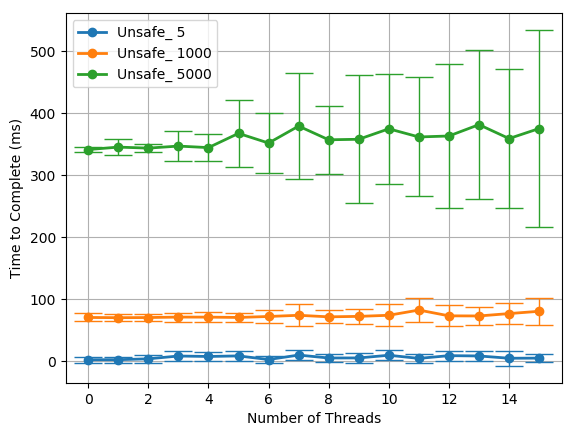
\includegraphics[scale=0.65]{step3_1.png}
\caption{Speed of the unsafe shared array when instantiated with various sizes}
\label{fig:step3_1}
\end{figure}


\begin{figure}
\centering
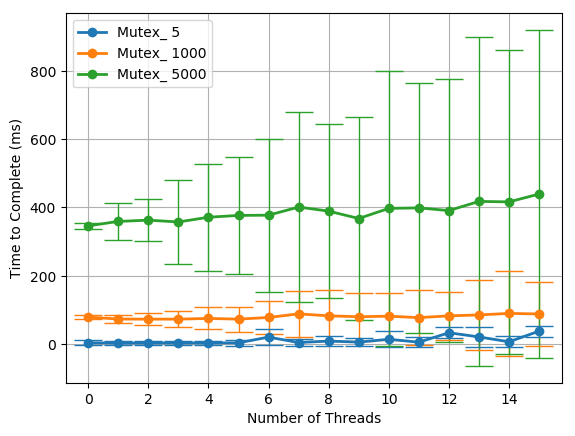
\includegraphics[scale=0.65]{step3_2.png}
\caption{Speed of the safe, mutex locked, shared array when instantiated with various sizes}
\label{fig:step3_2}
\end{figure}

The locked array (Fig \ref{fig:step3_2}) did not perform significantly worse in the average case than the unsafe array (Fig \ref{fig:step3_1}),
however the variance increases significantly as the number of threads and size of the array increases. I expect this is due to the existence of a one sided distribution. The majority of results are scattered close to the mean, however a small proportion of results were delayed significantly longer due to particularly long waits to acquire locks or worst case cache transactions. The difference in standard deviation and means for the largest array size is shown in Fig \ref{fig:step3_3}. The fact that the mean time to complete does not increase substantially with increasing thread count suggests that the bottleneck for each loop in the common case is not taking the lock or running the sum operation but instead due to overheads like loading the array to cache to be summed and checking exit conditions for the loop.

\begin{figure}
\centering
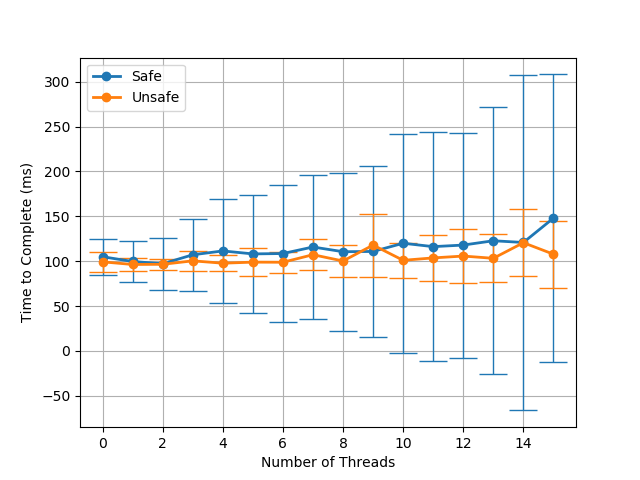
\includegraphics[scale=0.65]{step3_3.png}
\caption{Comparative speed of the unsafe and mutex-locked arrays set to a size of $X=5000$. The standard deviation is much more constant for the unsafe version.}
\label{fig:step3_3} 
\end{figure}


\subsection{TATAS Lock}

\begin{figure}
\centering
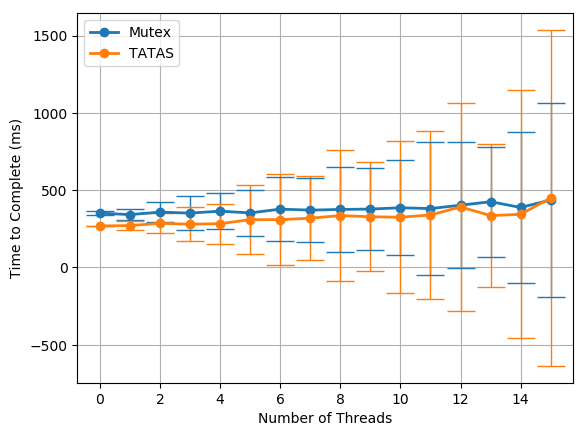
\includegraphics[scale=0.65]{step4_1.png}
\caption{Speed of the mutex-locked and TaTaS shared arrays for $X=5000$}
\label{fig:step4_1}
\end{figure}


The TaTaS-lock performed slightly better than the mutex-lock for small numbers of threads , but as the number increased, the performance of the TaTaS lock deteriorated and the standard deviation of its operation increased greatly (Fig \ref{fig:step4_1}). An explanation might be that the TaTaS's forecasted better cache-line behaviour works when relatively few threads are trying to take the mutual exclusion lock, but as the number of threads increases, so does the contention on the cache-coherence protocols, since test-and-test-and-set requires more cache coherency transactions than test-and-set. Furthermore, since the naive mutex lock simply uses Java's built-in \texttt{synchronized} primitive while the TaTaS was built using an \texttt{AtomicBoolean} and compare-and-set. The primitive must be able to lock over the whole object and hence may have some overhead in low-contention cases, but by being built-in, it may be able to take advantage of more low level JVM optimisations in higher contention cases. The high-level TaTaS construction is built with more general constructs, making it harder for the JVM to optimise away.

\subsection{Reader-Writer Lock}
\begin{figure}
\centering
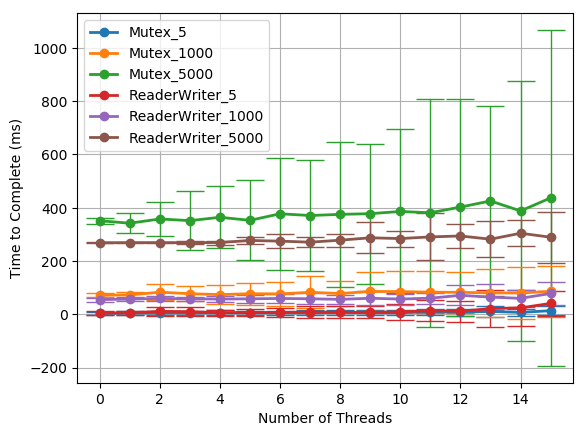
\includegraphics[scale=0.65]{step5_1.png}
\caption{Speed of the mutex-locked array versus the reader-writer locked array when instantiated with various sizes}
\label{fig:step5_1}
\end{figure}

\begin{figure}
\centering
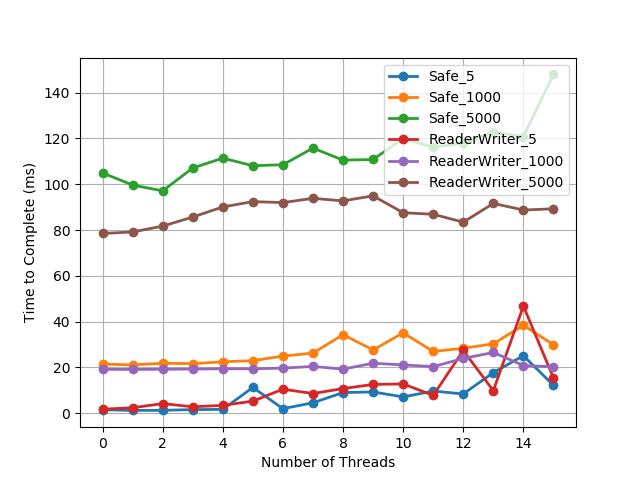
\includegraphics[scale=0.65]{step5_2.png}
\caption{Speed of the mutex-locked array versus the reader-writer locked array when instantiated with various sizes, drawn without error bars to more clearly show the mean-behaviour.}
\label{fig:step5_2}
\end{figure}

When the array size is not negligibly small, the reader-writer lock significantly outperforms the standard mutex lock. It also has a much smaller standard deviation for each operation than seen in mutex case (Figs \ref{fig:step5_1}, \ref{fig:step5_2}). Firstly, the reader-writer lock allows as many writers as possible to access the array. Secondly, the maximum wait time for a thread to access the array would be much shorter due to fewer pathological cases where lots of threads are blocked on each other. This means that the distribution of run-times would be much smaller.


\subsection{Flag-Based Lock}

\begin{figure}
\centering
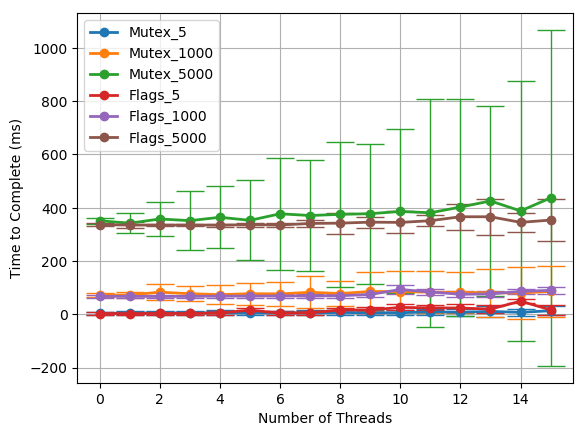
\includegraphics[scale=0.65]{step6_1.png}
\caption{Speed of the mutex-locked array versus the flag-locked array when instantiated with various sizes}
\label{fig:step6_1}
\end{figure}

The flag based lock outperformed the mutex-lock less significantly than the reader-writer lock but with an even tighter standard deviation. This may be due to the fact that the reader flags occupy separate cache lines, so there is even less delay in taking a read lock, as there is single memory location for there to be contention over (a single counter in the reader-writer case). This means that no threads have to compete for exclusive cache-line ownership of the lock, so the locking-time is improved.

\begin{figure}
\centering
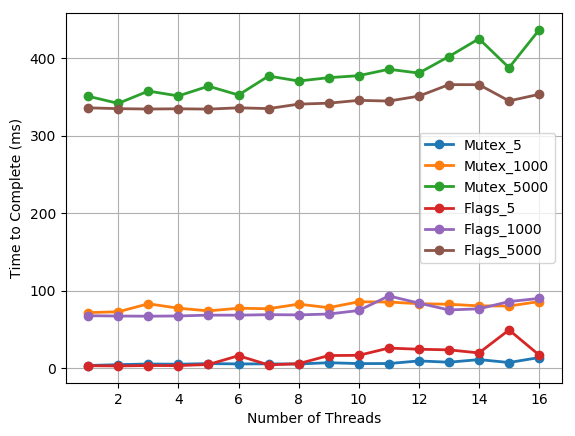
\includegraphics[scale=0.65]{step6_2.png}
\caption{Speed of the mutex-locked array versus the flag-locked array when instantiated with various sizes, drawn without error bars to more clearly show the mean-behaviour.}
\label{fig:step6_2}
\end{figure}

\subsection{Write Mode}


For the write-mode experiments, I fixed the array size to be $X = 1000$. Further more, since all experiments up to this point had been run to make 100,000 calls to the \texttt{sum} function in the main thread before halting, running a writing\texttt{update} operation every 100k iterations would have resulted in barely any write operations. Hence I decided to deviate from the specification and run \texttt{update}s every 10,000 iterations in the sparse update case.
In the frequent update case, I kept $K=100$ as specified. Despite iterating several times over reformulating the tests to remove experimental error, experimental results were still somewhat unstable from test run to test run. One factor appeared to be individual tests being greatly slowed due to environment processes, leading to anomalous spikes. The write tests appeared to be much more numerically unstable than the read-only tests.
\begin{figure}
\centering
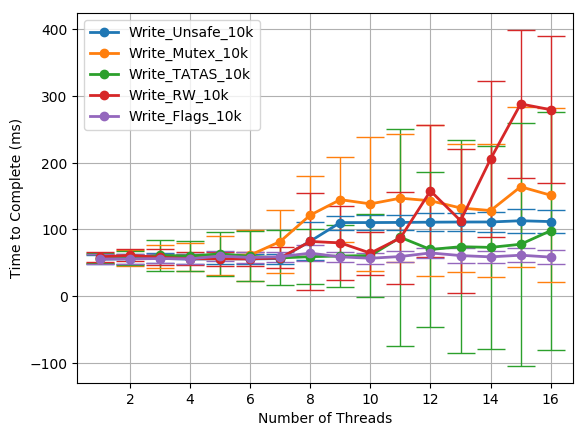
\includegraphics[scale=0.65]{step7_1.png}
\caption{Performance of each type of lock when used for update operations every 10,000 operations.}
\label{fig:step7_1}
\end{figure}

\begin{figure}
\centering
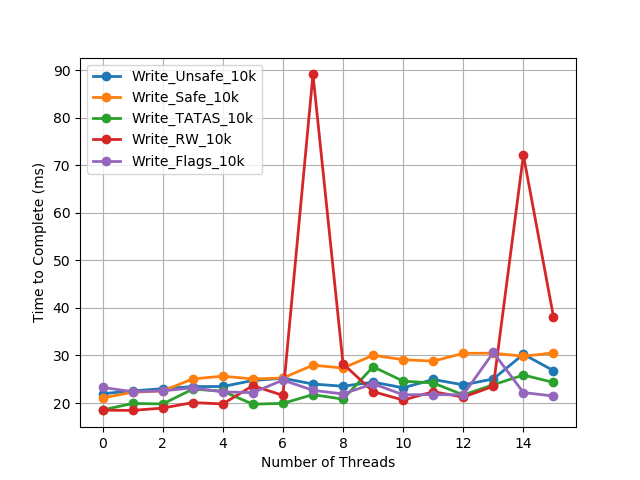
\includegraphics[scale=0.65]{step7_2.png}
\caption{Performance of each type of lock when used for update operations every 10,000 operations, drawn without error bars to more clearly show the mean-behaviour.}
\label{fig:step7_2}
\end{figure}



In the sparse update case ($k = 10,000$, Figs \ref{fig:step7_1}, \ref{fig:step7_2}), the best performer, as might be expected, was the flag based lock. This provided the least contention when switching between read and write locking. All five locking techniques performed well when the number of program threads was less than the number of hardware threads. Around and above 8 threads, performance deteriorated for most of the schemes. The unsafe case slowed to a very consistent speed over 8 threads. This may have been due to poor cache behaviour where threads were allowed to modify cache lines that were shared between other processors' caches. The basic mutex slowed more greatly and less predictably, likely due to its overzealous locking of read threads. The fact that we see a more obvious progression of runs getting slower as the number of threads increases compared with the read-only tests may be due to the JVM or bare metal processor itself enforcing a total store order on the write operations to the same address. This means that fewer runtime optimisations such as memory instruction reordering available, making performance more predictable. The reader-writer lock performed poorly and inconsistently. This may be due to a high level of contention on the atomic integer that represents the lock. This lock is continuously atomically \texttt{Compare-And-Set}ed by multiple threads at once. The TaTaS lock performed well due to its better cache behaviour over the mutex. This presents questions as one would expect it to have similar cache behaviour to the reader-writer lock.

\begin{figure}
\centering
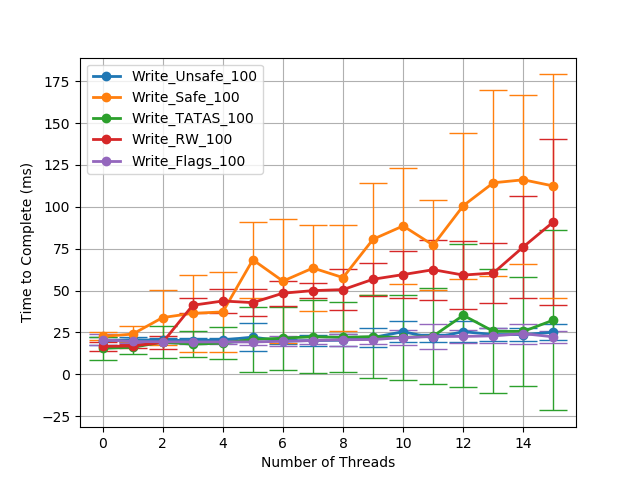
\includegraphics[scale=0.65]{step7_3.png}
\caption{Performance of each type of lock when used for update operations every 100 operations}
\label{fig:step7_3}
\end{figure}

\begin{figure}
\centering
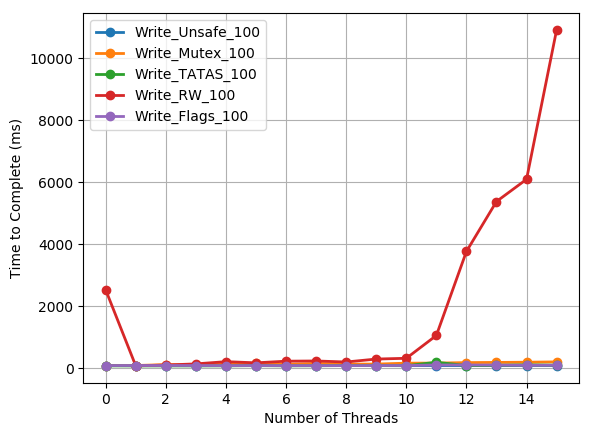
\includegraphics[scale=0.65]{step7_4.png}
\caption{Performance of each type of lock when used for update operations every 100 operations, drawn without error bars to more clearly show the mean-behaviour.}
\label{fig:step7_4}
\end{figure}

These trends continue for the more frequent update case. The Reader-Writer and simple mutex locks continued to be the least performant, showing poor run-times from a lower thread count in this case. The unsecured case continued to provide a consistent level of performance that was worse than the best locked cases, and the TaTaS and Flags based locks continued to run fastest, with the Flag-Lock also having a very low variance.

\section{Summary}

One issue with these experiments has been the non-reproducibility of the tests. Despite the high number of repeats (200 tests per batch) and length of tests in terms of operations (100k operations per test), and reviews of my experimental methods, I have seen poor reproducibility, most obviously in running the \texttt{update} operation tests. Another anomaly is the general lack of performance degradation as the number of threads increased. In each test case, we would expect the amount of time to complete to increase by around a factor of two between 8 threads and 16, however this has not occurred. This suggests there is an additional overhead in the tests brought about by the operation of the JVM. Further more, since Java is a higher level language and there a large number of techniques used to make the JVM run fast, such as JIT compilation, performance can be hard to predict. Perhaps using a lower level language such as C or C++ with compiler optimisations turned off might cause trends to be more obvious.

\end{document}